\documentclass[../notes.tex]{subfiles}
\graphicspath{{\subfix{../img/}}}
\begin{document}

\section{Linear Control Methods}
\subsection{Open Loop}
The system identification reveals how the inputs affect the outputs and the state of the system. We can work backwards from the desired output to find the required input. 
\paragraph{Example} In the context of a car's cruise control, we would like to achieve a desired speed with our throttle input. With a model of the car, we can determine the effect of the factors at play in the system: Throttle response, engine force, drag force, tire friction, etc. Treating the system as an equation and solving through, the throttle input required can be solved.
\subsection{Closed Loop (Feedback)}
\begin{figure}[H]
    \centering
    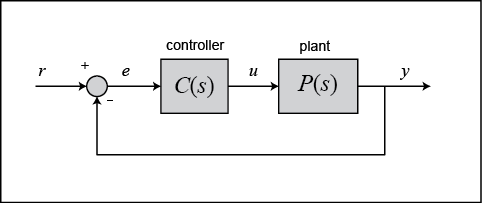
\includegraphics[width=0.7\linewidth]{feedback_block.png}
    \caption{Block Diagram of Feedback Loop}
    \label{fig:feedbackBlock}
\end{figure}
\paragraph{Example} Returning to the example of the cruise control, imagine that the same system (plant + controller) encounters a hill. Climbing up the slope changes the effect of the gravity force, meaning that our previous throttle input is not longer bringing the desired results. If a feedback system is implemented, the error between the desired speed and the actual speed can be calculated. With this information available, we can design our controller to account for disturbances, such as that hill.

\paragraph{Disturbance Modeling}
In between the plant and the output, disturbances in the system are modeled. An example of a disturbance is the hill previously discussed, but it can also include modeling uncertainties / inaccuracies in the plant.

\subsubsection{Purpose}
\begin{emphasis} \label{sec:feedbackMyopia}
   $\boxed{\text{Note:}}$ Feedback control systems may be myopic! In many designs, they do not have the information or sophistication to understand that current decisions might make control of the vehicle impossible later on!
\end{emphasis}

\subsection{Bode Plots}
The Bode plot is way to visualize the transfer function of a system. The Bode plot is a pair of subplots that show the magnitude and phase of a transfer function evaluated for $s-i\omega$ over the interval $\omega \in (0, \infty)$. In other words, it is the 3D magnitude and phase surface sliced along the positive $i\omega$-axis. Bode plots are helpful for understanding the steady-state behavior, as it shows the amplification factor and phase shift that the system will exhibit relative to a sinusoidal persistent input.\\ 
Bode plots are shown on logarithmic scales, using the product property for ease.
\paragraph{Logarithm Product Property}
\begin{equation*}
    \log(a\cdot b) = \log(a) + \log(b)
\end{equation*}

\paragraph{Geometry of Transfer Functions}
Transfer functions  are usually expressed as fractions of polynomials.
\begin{equation*}
    T(s) = k \cdot \frac{\prod_{i=1}(s-z_i)}{\prod_{i=1}(s-p_i)}
\end{equation*}
Splitting up these complex numbers using Euler's formula (\underline{\ref{eq:euler_form}}), we can separate the magnitude and phase of the transfer function.
\begin{align*}
    \text{Magnitude: } |T(s)| &= |k| \cdot \frac{\prod_{i=1}|s-z_i|}{\prod_{i=1}|s-p_i|} \\
    \text{Phase: } \angle T(s) &= \angle k + \sum_{i=1} \angle(s-z_i) - \sum_{i=1} \angle(s-p_i)
\end{align*}
These are then plotted on a log scale, after taking the base-10 logarithm and multiplying by 20.
\begin{equation*}
    20\log_{10}|T(s)| = 20\log_{10}|k| + 20\sum_{i=1}\log_{10}|s-z_i| - 20\sum_{i=1}\log_{10}|s-p_i|
\end{equation*}

\subsection{PID Control}
The PID controller is one of the simplest types of controllers.
\begin{description}
    \item[Proportional Gain (P term)] Applies a control input proportional to the amount of error.
    \item[Integral Gain (I term)] Applies a control input proportional to the integral of error (sum of error over time). This term is useful for countering steady-state error.
    \item[Derivative Gain (D term)] Applies a control input proportional to the rate of change of the error. This term is useful for countering overshoot.
\end{description}

\begin{figure}[H]
    \centering
    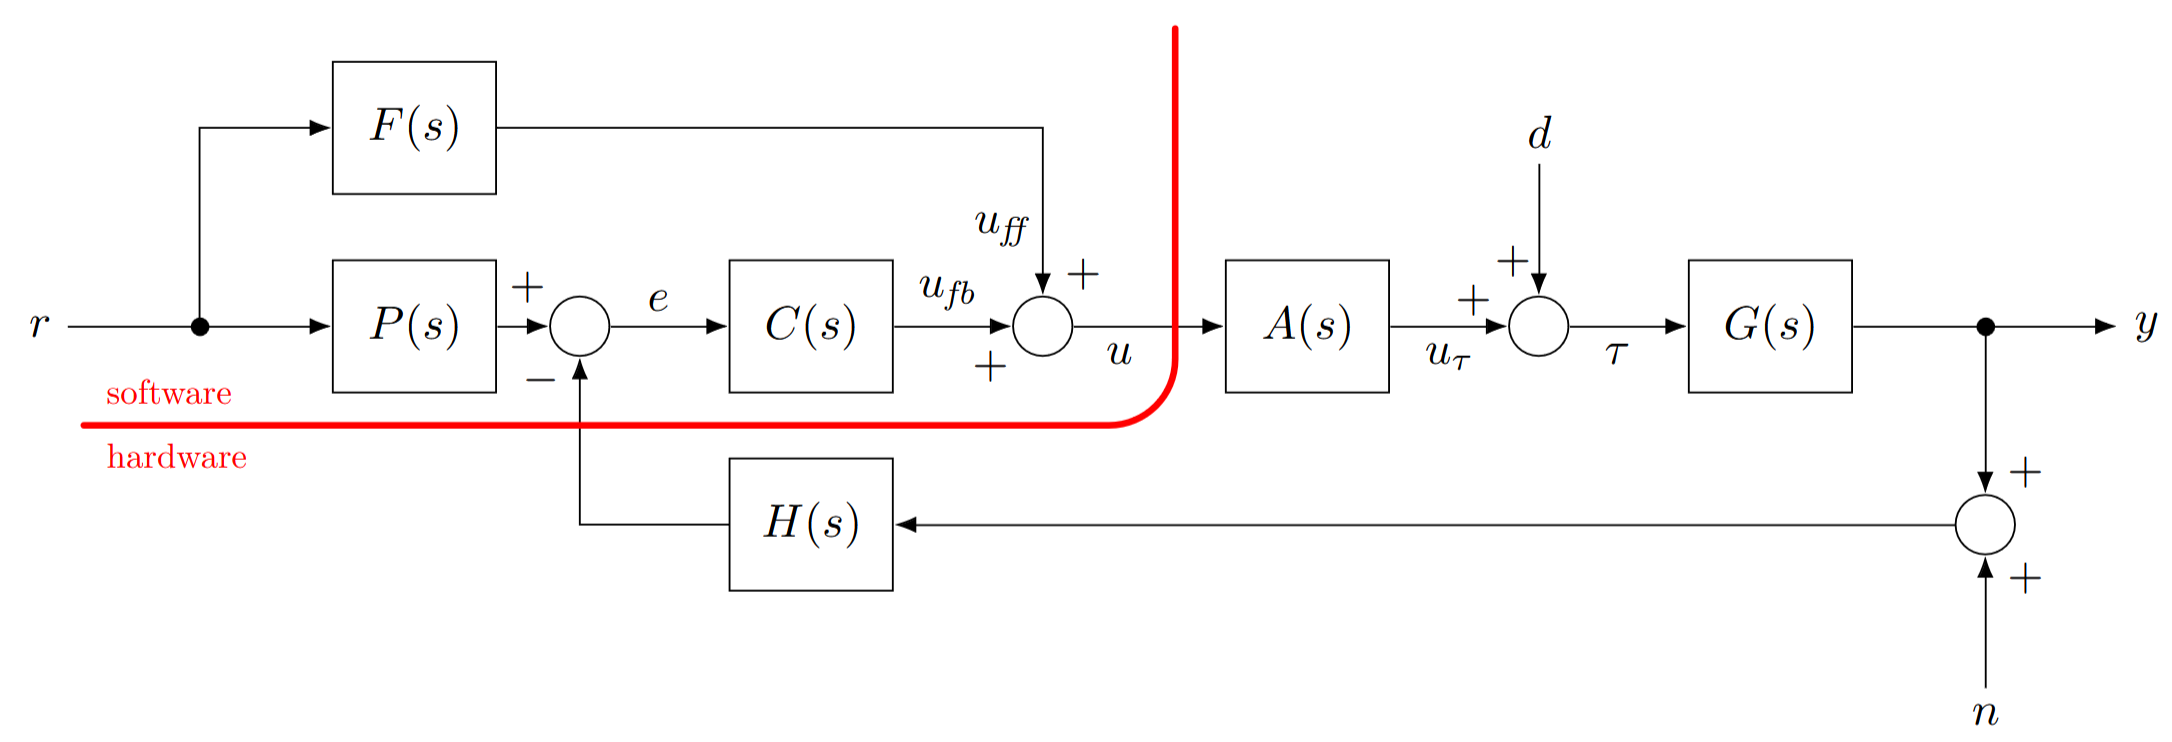
\includegraphics[width=1\linewidth]{block.png}
    \caption{Typical Control Block Diagram for Feedback System}
    \label{fig:typicalBlock}
\end{figure}

The PID controller can also be represented as a transfer function.
\begin{equation} \label{eq:PIDTF}
    K_p + \frac{K_i}{s} + K_d s = \frac{K_ds^2 + K_ps + K_i}{s}
\end{equation}

\subsubsection{Gain Margin}
\paragraph{Amplification Gain Margin}
\paragraph{Attenuation Gain Margin}

\subsubsection{Phase Margin}

\subsubsection{Crossover Frequency}
\paragraph{Gain Crossover Frequency}
\paragraph{Phase Crossover Frequency}



\subsubsection{Integrator Anti-windup Term}
In certain cases where the error does not correct rapidly, the I term may "wind up" (error over time builds up, resulting in large corrections). The large correction applied may destabilize the system. To counter this, an "anti-windup" term can be used, to limit the sum of error the integral term sees.
\paragraph{Example}

\subsection{Higher-order Controllers}
\subsubsection{Lead-Lag Control}
\subsection{Feedforward}
Feedforward control can address some of the drawbacks of feedback control, such as the case of myopia (\underline{\ref{sec:feedbackMyopia}}). For this reason, feedforward is sometimes referred to as guidance.

\subsection{Multi-Input, Multi-Output (MIMO)}
So far, all of the techniques have addressed mainly single input, single output systems (SISO).

\subsection{Designing the Controller}

\subsubsection{Frequency Response Method}
\subsubsection{Root Locus Method}


\subsubsection{Loop-Shaping Method}
Loop-shaping is somewhat of an enhancement to the frequency response method, using the Nyquist plot in addition to the Bode plot.

\subsubsection{Examples}
\paragraph{PID Tuning}
Take Figure \ref{fig:typicalBlock} as the block diagram for the example system for which the PID controller is being tuned.

A PID controller is designed to satisfy the following requirements: A loop gain crossover frequency of 1 Hz, an amplification gain margin of 6dB or better, an attenuation gain margin of 10dB or better, and a phase margin of $45^{\circ}$ or better.


\end{document}